\documentclass{standalone}
\usepackage{tikz}
\usetikzlibrary{patterns, positioning}

\begin{document}
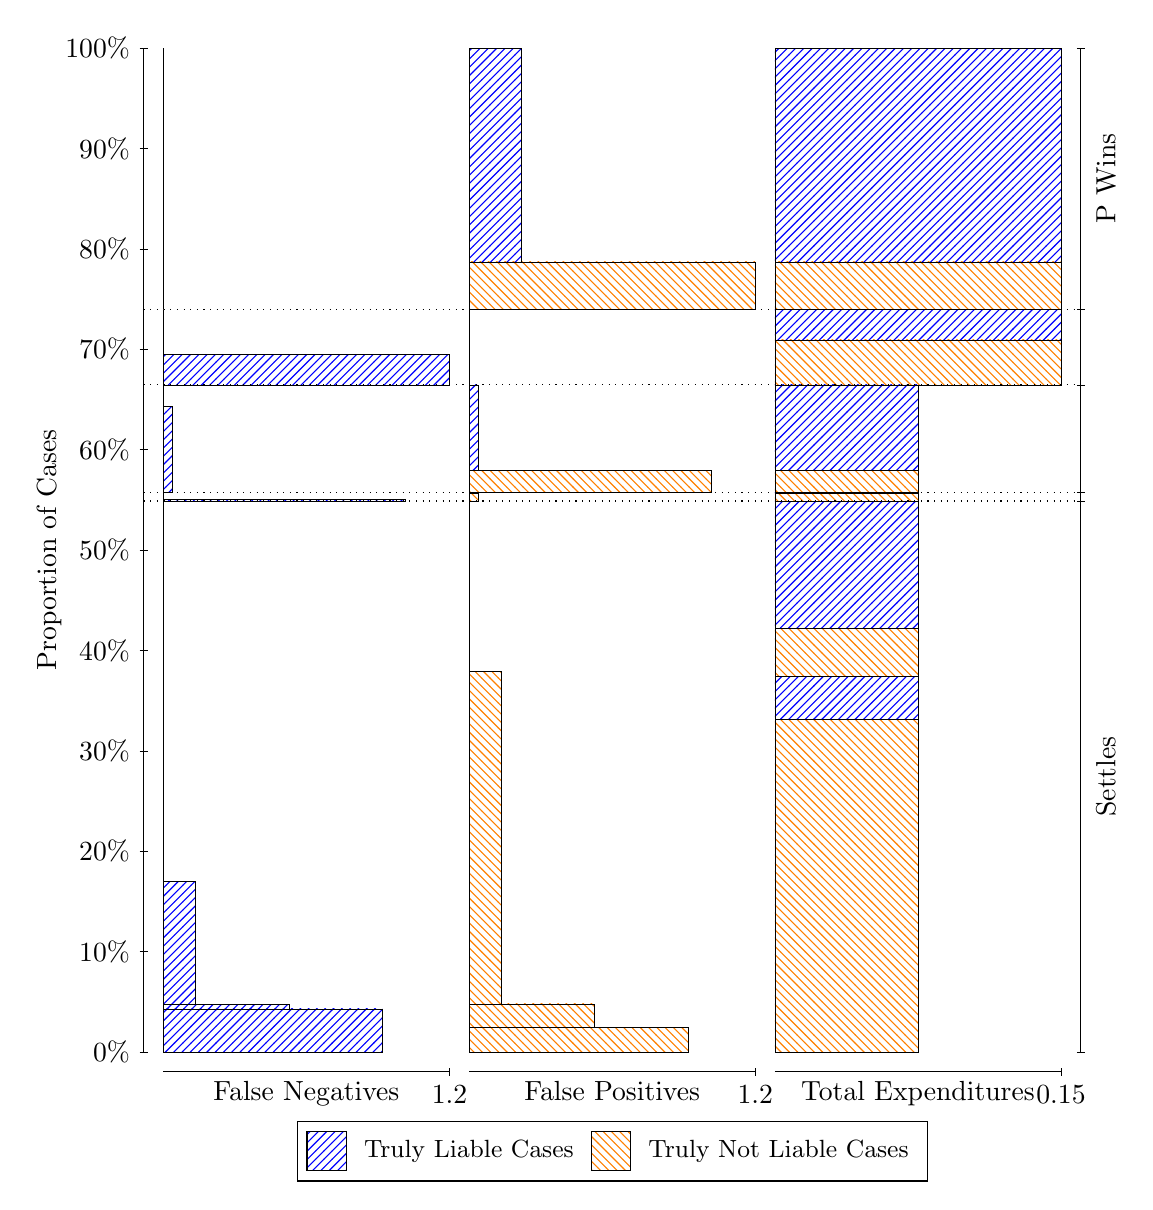
\begin{tikzpicture}
\draw[black, very thin] (1.5,1.75) -- (1.5,14.5);
\node[rotate=90, anchor=center] at (0.3, 8.125) {Proportion of Cases};
\draw[black, very thin] (1.45,1.75) -- (1.55,1.75);
\node[anchor=east] at (1.45, 1.75) {0\%};
\draw[black, very thin] (1.45,3.025) -- (1.55,3.025);
\node[anchor=east] at (1.45, 3.025) {10\%};
\draw[black, very thin] (1.45,4.3) -- (1.55,4.3);
\node[anchor=east] at (1.45, 4.3) {20\%};
\draw[black, very thin] (1.45,5.575) -- (1.55,5.575);
\node[anchor=east] at (1.45, 5.575) {30\%};
\draw[black, very thin] (1.45,6.85) -- (1.55,6.85);
\node[anchor=east] at (1.45, 6.85) {40\%};
\draw[black, very thin] (1.45,8.125) -- (1.55,8.125);
\node[anchor=east] at (1.45, 8.125) {50\%};
\draw[black, very thin] (1.45,9.4) -- (1.55,9.4);
\node[anchor=east] at (1.45, 9.4) {60\%};
\draw[black, very thin] (1.45,10.675) -- (1.55,10.675);
\node[anchor=east] at (1.45, 10.675) {70\%};
\draw[black, very thin] (1.45,11.95) -- (1.55,11.95);
\node[anchor=east] at (1.45, 11.95) {80\%};
\draw[black, very thin] (1.45,13.225) -- (1.55,13.225);
\node[anchor=east] at (1.45, 13.225) {90\%};
\draw[black, very thin] (1.45,14.5) -- (1.55,14.5);
\node[anchor=east] at (1.45, 14.5) {100\%};

\draw[black, very thin] (13.4,1.75) -- (13.4,14.5);
\draw[black, very thin] (13.35,1.75) -- (13.45,1.75);
\node[anchor=west] at (13.35, 1.75) {};
\draw[black, very thin] (13.35,8.7473) -- (13.45,8.7473);
\node[anchor=west] at (13.35, 8.7473) {};
\draw[black, very thin] (13.35,8.86) -- (13.45,8.86);
\node[anchor=west] at (13.35, 8.86) {};
\draw[black, very thin] (13.35,10.222) -- (13.45,10.222);
\node[anchor=west] at (13.35, 10.222) {};
\draw[black, very thin] (13.35,11.182) -- (13.45,11.182);
\node[anchor=west] at (13.35, 11.182) {};
\draw[black, very thin] (13.35,14.5) -- (13.45,14.5);
\node[anchor=west] at (13.35, 14.5) {};

\draw[black, very thin, pattern color=blue, pattern=north east lines] (1.75,1.75) rectangle (4.5306,2.2979);
\draw[black, very thin, pattern color=blue, pattern=north east lines] (1.75,2.2979) rectangle (3.3442,2.3582);
\draw[black, very thin, pattern color=blue, pattern=north east lines] (1.75,2.3582) rectangle (2.1578,3.9152);
\draw[black, very thin, pattern color=orange, pattern=north west lines] (1.75,3.9152) rectangle (1.75,8.7473);
\draw[black, very thin, pattern color=blue, pattern=north east lines] (1.75,8.7473) rectangle (4.8272,8.7676);
\draw[black, very thin, pattern color=orange, pattern=north west lines] (1.75,8.7676) rectangle (1.75,8.86);
\draw[black, very thin, pattern color=blue, pattern=north east lines] (1.75,8.86) rectangle (1.8612,9.944);
\draw[black, very thin, pattern color=orange, pattern=north west lines] (1.75,9.944) rectangle (1.75,10.222);
\draw[black, very thin, pattern color=blue, pattern=north east lines] (1.75,10.222) rectangle (5.3833,10.612);
\draw[black, very thin, pattern color=orange, pattern=north west lines] (1.75,10.612) rectangle (1.75,11.182);
\draw[black, very thin, pattern color=orange, pattern=north west lines] (1.75,11.182) rectangle (1.75,11.783);
\draw[black, very thin, pattern color=blue, pattern=north east lines] (1.75,11.783) rectangle (1.75,14.5);
\draw[black, very thin, pattern color=orange, pattern=north west lines] (5.6333,1.75) rectangle (8.4139,2.0621);
\draw[black, very thin, pattern color=orange, pattern=north west lines] (5.6333,2.0621) rectangle (7.2276,2.3618);
\draw[black, very thin, pattern color=orange, pattern=north west lines] (5.6333,2.3618) rectangle (6.0412,6.5822);
\draw[black, very thin, pattern color=blue, pattern=north east lines] (5.6333,6.5822) rectangle (5.6333,8.7473);
\draw[black, very thin, pattern color=orange, pattern=north west lines] (5.6333,8.7473) rectangle (5.7446,8.8397);
\draw[black, very thin, pattern color=blue, pattern=north east lines] (5.6333,8.8397) rectangle (5.6333,8.86);
\draw[black, very thin, pattern color=orange, pattern=north west lines] (5.6333,8.86) rectangle (8.7105,9.1385);
\draw[black, very thin, pattern color=blue, pattern=north east lines] (5.6333,9.1385) rectangle (5.7446,10.222);
\draw[black, very thin, pattern color=orange, pattern=north west lines] (5.6333,10.222) rectangle (5.6333,10.793);
\draw[black, very thin, pattern color=blue, pattern=north east lines] (5.6333,10.793) rectangle (5.6333,11.182);
\draw[black, very thin, pattern color=orange, pattern=north west lines] (5.6333,11.182) rectangle (9.2667,11.783);
\draw[black, very thin, pattern color=blue, pattern=north east lines] (5.6333,11.783) rectangle (6.3007,14.5);
\draw[black, very thin, pattern color=orange, pattern=north west lines] (9.5167,1.75) rectangle (11.333,5.9703);
\draw[black, very thin, pattern color=blue, pattern=north east lines] (9.5167,5.9703) rectangle (11.333,6.5182);
\draw[black, very thin, pattern color=orange, pattern=north west lines] (9.5167,6.5182) rectangle (11.333,7.1301);
\draw[black, very thin, pattern color=blue, pattern=north east lines] (9.5167,7.1301) rectangle (11.333,8.7473);
\draw[black, very thin, pattern color=orange, pattern=north west lines] (9.5167,8.7473) rectangle (11.333,8.8397);
\draw[black, very thin, pattern color=blue, pattern=north east lines] (9.5167,8.8397) rectangle (11.333,8.86);
\draw[black, very thin, pattern color=orange, pattern=north west lines] (9.5167,8.86) rectangle (11.333,9.1385);
\draw[black, very thin, pattern color=blue, pattern=north east lines] (9.5167,9.1385) rectangle (11.333,10.222);
\draw[black, very thin, pattern color=orange, pattern=north west lines] (9.5167,10.222) rectangle (13.15,10.793);
\draw[black, very thin, pattern color=blue, pattern=north east lines] (9.5167,10.793) rectangle (13.15,11.182);
\draw[black, very thin, pattern color=orange, pattern=north west lines] (9.5167,11.182) rectangle (13.15,11.783);
\draw[black, very thin, pattern color=blue, pattern=north east lines] (9.5167,11.783) rectangle (13.15,14.5);
\draw[black, dotted] (1.5,8.7473) -- (13.4,8.7473);
\draw[black, dotted] (1.5,8.86) -- (13.4,8.86);
\draw[black, dotted] (1.5,10.222) -- (13.4,10.222);
\draw[black, dotted] (1.5,11.182) -- (13.4,11.182);
\draw[black, very thin] (1.75,1.5) -- (5.3833,1.5);
\node[anchor=north] at (3.5667, 1.5) {False Negatives};
\draw[black, very thin] (5.3833,1.45) -- (5.3833,1.55);
\node[anchor=north] at (5.3833, 1.45) {1.2};

\draw[black, very thin] (5.6333,1.5) -- (9.2667,1.5);
\node[anchor=north] at (7.45, 1.5) {False Positives};
\draw[black, very thin] (9.2667,1.45) -- (9.2667,1.55);
\node[anchor=north] at (9.2667, 1.45) {1.2};

\draw[black, very thin] (9.5167,1.5) -- (13.15,1.5);
\node[anchor=north] at (11.333, 1.5) {Total Expenditures};
\draw[black, very thin] (13.15,1.45) -- (13.15,1.55);
\node[anchor=north] at (13.15, 1.45) {0.15};

\node[black, centered, rotate=90] at (13.72, 5.2487) {Settles};



\node[black, centered, rotate=90] at (13.72, 12.841) {P Wins};

\draw (7.449999999999999,1.5) node[draw=none] (baseCoordinate) {};
\begin{scope}[align=center]
        \matrix[scale=0.5, draw=black, below=0.5cm of baseCoordinate, nodes={draw}, column sep=0.1cm]{
            \node[rectangle, draw, minimum width=0.5cm, minimum height=0.5cm, pattern=north east lines, pattern color=blue] {}; &
            \node[draw=none, font=\small] (B) {Truly Liable Cases}; &
            \node[rectangle, draw, minimum width=0.5cm, minimum height=0.5cm, pattern=north west lines, pattern color=orange] {}; &
            \node[draw=none, font=\small] (B) {Truly Not Liable Cases}; \\
            };
\end{scope}

\end{tikzpicture}
\end{document}